\documentclass[a4paper, 12pt]{article}

\newcommand{\assignmentAuthor}{Bhaskar Goyal}
\newcommand{\course}{CSCI - 567}
\newcommand{\assignmentName}{HW 01}
\newcommand{\USCID}{6547367383}
\newcommand{\assignmentDate}{July 3, 2021}

\addtolength{\hoffset}{-2.25cm}
\addtolength{\textwidth}{4.5cm}
\addtolength{\voffset}{-2.5cm}
\addtolength{\textheight}{5cm}
\setlength{\parskip}{0pt}
\setlength{\parindent}{15pt}

\usepackage{amsthm}
\usepackage{amsmath}
\usepackage{amssymb}
\usepackage{bm}
\usepackage[colorlinks = true, linkcolor = black, citecolor = black, final]{hyperref}
\usepackage{tikz}
\usetikzlibrary{automata}

\usepackage{graphicx}
\usepackage{multicol}
\usepackage{ marvosym }
\usepackage{wasysym}
\usepackage{tikz}
\usetikzlibrary{patterns}
\usepackage{fancyhdr}
\usepackage{amssymb,latexsym,amsmath,amsthm}
\usepackage{amsfonts,rawfonts}
\usepackage{thmtools}
\usepackage{systeme}
\usepackage{mathtools}

\pagestyle{fancy}
\fancyhf{}
\rhead{\assignmentAuthor \; (USC ID - \USCID)}
\lhead{\course \; \assignmentName}
\rfoot{Page \thepage}
\lfoot{\assignmentDate}

\newcommand{\ds}{\displaystyle}

\setlength{\parindent}{0in}

\declaretheoremstyle[
headfont=\color{blue}\normalfont\bfseries,
notefont=\bfseries, 
notebraces={}{},
% bodyfont=\color{red}\normalfont\itshape,
bodyfont=\normalfont,%\itshape,
%headformat=\NUMBER.~\NAME\NOTE
headformat=\NAME\NOTE
]{colorquestion}

\declaretheorem[
numbered=no,
style=colorquestion,
name=Question
]{question}

\title{\course \; \assignmentName}
\author{\textbf{\assignmentAuthor} \\ \Small{USC ID - \USCID}}
\date{\assignmentDate}

% ----------------------------

% The "stuff" above here is called the preamble of the document.  It sets the margins and loads special packages.  Probably the only reason you would need to edit something above here would be to add a package to do something very specific... but probably everything you need is loaded already

% -----------------------------

\begin{document}
\thispagestyle{plain}
\maketitle
\hrule
\bigskip

% -------------------------
% Question 1
% -------------------------

\begin{question}[1]
Arrange the following functions in increasing order of growth rate with $g(n)$ following
\(f(n)\) in your list if and only if \(f(n) = O(g(n))\)
\bigskip
\begin{align*}
    2^{\log n},\hspace{2em}
    (\sqrt{2})^{\log n},\hspace{2em}
    n (\log n)^3,\hspace{2em}
    2^{\sqrt{2 \log n}},\hspace{2em}
    2^{2^n},\hspace{2em}
    n \log n,\hspace{2em}
    2^{n^2}
\end{align*}
\smallskip
\end{question}

\begin{proof}[\color{red}{Solution}]
Comparing all the values one by one
\smallskip

(1) \hspace{1em} 
\begin{align*}
    2^{\log n} &= n \\
    &= O(n)
\end{align*}

(2) \hspace{1em} 
\begin{align*}
    (\sqrt{2})^{\log n} &= 2^{\frac{\log n}{2}} \\
    &= 2^{\frac{1}{2} \log n} \\
    &= 2^{\log n^\frac{1}{2}} && \text{\footnotesize } \\
    &= n^{\frac{1}{2}} \\
    &= \sqrt{n} \\
    &= O(\sqrt{n})
\end{align*}

(3) \hspace{1em} 
\begin{align*}
    n (\log n)^3 &= O(n (\log n)^3) \\
\end{align*}

(4) \hspace{1em} 
Comparing $2^{\sqrt{2 \log n}}$ with $n$ using L' Hospital Rule
\begin{align*}
    \lim_{n \to \infty} \frac{f(n)}{g(n)} &= \frac{f^{'}(n)}{g^{'}(n)} \\
    &= \frac{\frac{d(2^{\sqrt{2 \log n}})}{d n}}{\frac{d(n)}{d n}} \\
    &= \to 0
\end{align*}

\hspace{4em} So, $2^{\sqrt{2 \log n}} < n$

\hspace{4em} Comparing $2^{\sqrt{2 \log n}}$ with $\sqrt{n}$ using L' Hospital Rule
\begin{align*}
    \lim_{n \to \infty} \frac{f(n)}{g(n)} &= \frac{f^{'}(n)}{g^{'}(n)} \\
    &= \frac{\frac{d(2^{\sqrt{2 \log n}})}{d n}}{\frac{d(\sqrt{n})}{d n}} \\
    &= \to 0
\end{align*}

\hspace{4em} So, $2^{\sqrt{2 \log n}} < \sqrt{n}$

\hspace{4em} Combining both the conclusions, \emph{$2^{\sqrt{2 \log n}} < \sqrt{n} < n$}

\bigskip
(5) \hspace{1em} 
Comparing $2^{2^n}$ with $2^{n^2}$, 

\hspace{4em} Both of the terms only have different exponent terms. So, we only need to compare the exponents. For $2^{2^n}$ is $2^n$ and for $2^{n^2}$ is $n^2$
\begin{align*}
    \text{Clearly, }  2^n &> n^2 
\end{align*}

\hspace{4em} So, $2^{2^n} > 2^{n^2}$

(6) \hspace{1em} 
\begin{align*}
    n (\log n) &= O(n (\log n)) \\
\end{align*}

(7) \hspace{1em} Already compared in $5^{th}$ point, as $2^{2^n} > 2^{n^2}$ 

\bigskip
Using all the above points the final answer is 

\begin{align*}
    \bm{2^{\sqrt{2 \log n}} < (\sqrt{2})^{\log n} < 2^{\log n} < n \log n < n (\log n)^3 < 2^{n^2} < 2^{2^n}} 
\end{align*}
\end{proof}



% -------------------------
% Question 2
% -------------------------
\hrule
\bigskip
\begin{question}[2]
Give a linear time algorithm based on BFS to detect whether a given undirected graph
contains a cycle. If the graph contains a cycle, then your algorithm should output one. It should
not output all cycles in the graph, just one of them. You are NOT allowed to modify BFS, but
rather use it as a black box. Explain why your algorithm has a linear time run-time complexity.

\end{question}

\begin{proof}[\color{red}{Solution}]
Algorithm can be run on graph $G$ in following steps below. 

\begin{enumerate}
    \item Run $BFS$ on a graph $G$, let the output edges of the graph be a set of edges be $S_{BFS}$. This can be achieved in $O(V + E)$
    \[ S_{BFS} \leftarrow BFS_{Output}  \tag*{\footnotesize O(V + E)} \\\]
    
    \item Prepare a set of all the edges in Graph $G$. Let that be $S_G$. This can be done in $O(E)$ for an adjacency list graph. 
    
    \item The edges which are not in $S_{BFS}$ but in $S_{G}$ are cyclic edges. To get these subtract $S_{BFS}$ from $S_G$. This can be achieved in $O(E)$
    \[ S_{Cyclic Edges} \leftarrow S_G - S_{BFS}  \tag*{\footnotesize O(E)} \\\]
    
    \item Let an edge in $S_{Cyclic Edges}$ be $(u, v)$. Get all the parent hierarchy of both $u$ and $v$ from $S_{BFS}$. Let that be $L_{u}$ and $L_{v}$. This can be achieved in $O(E)$.
    \[ L_{u} \leftarrow \text{Parent Hierarchy of $u$ from } S_{BFS}  \tag*{\footnotesize O(E)} \]
    \[ L_{v} \leftarrow \text{Parent Hierarchy of $v$ from } S_{BFS}  \tag*{\footnotesize O(E)} \]
    
    \item Find the first common ancestor in Both List $L_u$ and $L_v$. Let this be node $w$. (This can be done in $O(E)$ by traversing both the list in reverse and return the last common element).
    \[ w \leftarrow \text{first\_common\_ancestor($L_u$, $L_v$)} \tag*{\footnotesize O(E)} \]
    \[ L_{u ... w} \leftarrow \text{ Part of $L_u$ from u to w}  \]
    \[ L_{w ... v} \leftarrow \text{ Part of $L_v$ from w to v}  \tag*{\footnotesize (Reverse order)} \]
    
    \item The cycle can returned as $(L_{u ... w}, L_{w ... v})$
\end{enumerate}

The final run time complexity is \bm{$O(V + E)$} (linear time).
\bigskip

\textbf{\textit{Example: }}Let Graph $G$ be
\bigskip
\begin{center}
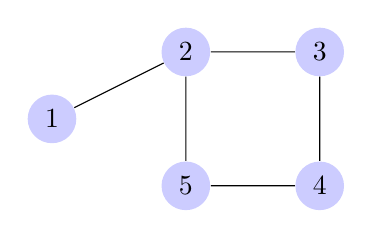
\begin{tikzpicture}  
  [scale=1.7,auto=center,every node/.style={circle,fill=blue!20}] % here, node/.style is the style pre-defined, that will be the default layout of all the nodes. You can also create different forms for different nodes.  
    
  \node (a1) at (1,4.5) {1};  
  \node (a2) at (2,5)  {2}; % These all are the points where we want to locate the vertices. You can create your diagram first on a rough paper or graph paper; then, through the points, you can create the layout. Through the use of paper, it will be effortless for you to draw the diagram on Latex.  
  \node (a3) at (3,5)  {3};  
  \node (a4) at (3,4) {4};  
  \node (a5) at (2,4)  {5}; 
  
  \draw (a1) -- (a2); % these are the straight lines from one vertex to another  
  \draw (a2) -- (a3);  
  \draw (a3) -- (a4);   
  \draw (a4) -- (a5);  
  \draw (a2) -- (a5);  
  
\end{tikzpicture} 

\end{center}

Running all the steps
\begin{enumerate}
    \item $S_{BFS}\leftarrow \; \{(1, 2), (2, 3), (2, 5), (3, 4)\}$
    \item $S_{G}\leftarrow \; \{(1, 2), (2, 3), (2, 5), (3, 4), (4,5)\}$
    \item $S_{Cyclic Edges} \leftarrow \; \{(4, 5)\}$ 
    \item \begin{align*}
        u &\leftarrow 4 \\
        v &\leftarrow 5 \\
        L_{u} &\leftarrow (3, 2, 1) \tag*{\footnotesize (Parent Hierarchy of u = 4)}\\
        L_{v} &\leftarrow (2, 1)
    \end{align*}
    \item \[ w \leftarrow 2 \tag*{\footnotesize First Common Ancestor} \]
    \[ L_{u ... w} \leftarrow \text{ (4, 3, 2)}  \]
    \[ L_{w ... v} \leftarrow \text{ (2, 5)}  \tag*{\footnotesize Reverse order} \]
    \item Cycle $\leftarrow$ (4, 3, 2, 5) \;\;\;\;\; ($\because$ \text{Combination of } $L_{u ... w}$ and  $L_{w ... v}$)
\end{enumerate}

\end{proof}



% -------------------------
% Question 3
% -------------------------
\hrule
\bigskip
\begin{question}[3]
A binary tree is a rooted tree in which each node has at most two children. Show by
{\itshape induction} that in any nonempty binary tree the number of nodes with two children is exactly one
less than the number of leaves
\end{question}

\begin{proof}[\color{red}{Solution}]
Proving the statement by induction.
\smallskip

\textbf{Base Case:}

\hspace{1em} For a binary tree with only 1 node.

\hspace{1em} Hence, the number of leaves are $L = 1$. And the Number of Nodes with two children are $N = 0$.

\hspace{1em} The base case is being satisfied, as $L - N = 1$.

\smallskip

\textbf{Inductive Hypothesis:}

\hspace{1em} Assuming a tree of $N$ nodes with exactly 2 children. And the number of leaves are $L$. The proof holds as $L - N = 1$.

\smallskip

\textbf{Inductive Step:}

\hspace{1em} Adding a single node to a tree of $N$ nodes with exactly 2 children. And the number of leaves are $L$. There can be 2 cases for that. 

\begin{enumerate}
    \item Adding the new node ($A$) to a node with 0 children. 
    \begin{center}
        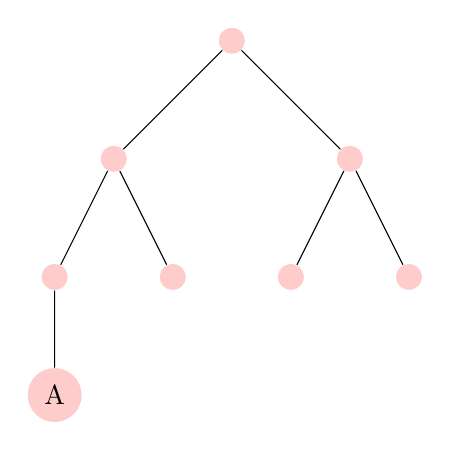
\begin{tikzpicture}[nodes={draw=none,circle,fill=red!20}]
          \node {}
            child { node {} 
                child { node {} 
                    child { node {A} }
                }
                child { node {} }
            }
            child [missing]
            child {node {} 
                child { node {} }
                child { node {} }
            };
        \end{tikzpicture}
    \end{center} 
    
    The number of Leaf Nodes = $L$\\
    The number of nodes with exactly 2 children = $N$. \\
    Still the equation $L - N = 1$ holds.
    
    \item Adding the new node ($A$) to a node with 1 children. 
    \begin{center}
        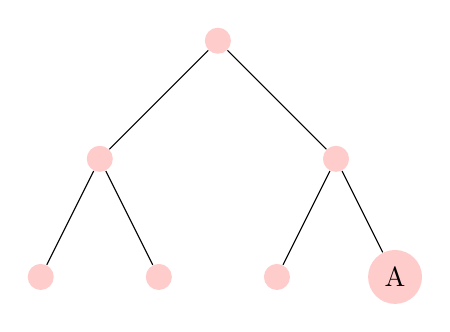
\begin{tikzpicture}[nodes={draw=none,circle,fill=red!20}]
          \node {}
            child { node {} 
                child { node {} }
                child { node {} }
            }
            child [missing]
            child {node {} 
                child { node {} }
                child { node {A} }
            };
        \end{tikzpicture}
    \end{center} 
    
    The number of Leaf Nodes = $L + 1$\\
    The number of nodes with exactly 2 children = $N + 1$. \\
    $\Rightarrow$ $(L + 1) - (N + 1) = 1$
    $\Rightarrow$ $L - N = 1$
\end{enumerate}

In both of the above cases, equation \bm{$L - N = 1$} holds. \textbf{Hence, proved}. 

\end{proof}



% -------------------------
% Question 4
% -------------------------
\hrule
\bigskip
\begin{question}[4]
Prove by contradiction that a complete graph $K_5$ is not a planar graph. You can use facts
regarding planar graphs proven in the textbook.
\end{question}

\begin{proof}[\color{red}{Solution}]
Proving by contradiction. 
\smallskip

Assume the graph $K_5$ is planar.

For all the planar graph, the theorem $E < 3V - 6$ holds. 
\smallskip

For a $K_5$ planar graph. \\
$E$ = 10 (number of Edges) \\
$V$ = 5 (number of Vertices) \\

Applying the $E < 3V - 6$,

\[ 10 < 3*5 - 6 \tag*{\footnotesize Applying theorem} \] 
\[ 10 \nless 9  \]

Because the theorem for planar graph does not hold true. Therefore, a complete graph $K_5$ is not a planar graph. \textbf{Hence, proved}
\end{proof}
\bigskip


% -------------------------
% Question 5
% -------------------------
\hrule
\bigskip
\begin{question}[5]
Suppose we perform a sequence of $n$ operations on a data structure in which the $i^{th}$
operation costs $i$ if $i$ is an exact power of 2, and 1 otherwise. Use aggregate analysis to determine
the amortized cost per operation
\end{question}

\begin{proof}[\color{red}{Solution}]
The cost per operation table is
\begin{center}
\begin{tabular}{ |c|c| } 
 \hline
 \textbf{\# Operation} & \textbf{Cost per Operation} \\
 \hline
 1 & 1 \\ 
 \hline
 2 & 2 \\ 
 \hline
 3 & 1 \\ 
 \hline
 4 & 4 \\ 
 \hline
 .. & .. \\ 
 \hline
 n - 1 & 1 \\ 
 \hline
 n (exact power of 2) & n \\ 
 \hline
\end{tabular}
\end{center}
\smallskip
Using the aggregate analysis 
\begin{align*} 
    \text{Amortized Cost} &= \frac{T(n)}{n} \\
    &= \frac{(1 + 2 + 4 + ... + n) + 1*(n-\log n))}{n} \\
    &= \frac{(2^{\log n} - 1) + n - \log n}{n} \tag*{\footnotesize  (Using Geometric Series Summation)} \\
    &= \frac{n + n - \log n - 1}{n} \\
    &= \frac{2n - \log n - 1}{n} \\
    &< \frac{2n}{n} \\
    &= \frac{O(2n)}{n} \\
    &= O(1)
\end{align*}

The Amortized Cost is \bm{$O(1)$}.


\end{proof}
\bigskip


% -------------------------
% Question 6
% -------------------------
\hrule
\bigskip
\begin{question}[6]
We have argued in the lecture that if the table size is doubled when it’s full, then the
amortized cost per insert is acceptable. Fred Hacker claims that this consumes too much space.
He wants to try to increase the size with every insert by just two over the previous size. What is
the amortized cost per insertion in Fred’s table?
\end{question}

\begin{proof}[\color{red}{Solution}]
The cost per operation table is
\begin{center}
\begin{tabular}{ |c|c|c|c| } 
 \hline
 \textbf{\# Operation} & \textbf{Old Size} & \textbf{New Size} & \textbf{Copy Operations}  \\
 \hline
 1 & 1 & & \\ 
 \hline
 2 & 1 & 3 & 1 \\ 
 \hline
 3 & 3 & & \\ 
 \hline
 4 & 3 & 5 & 3 \\ 
 \hline
 5 & 5 &  & \\ 
 \hline
 6 & 5 & 7 & 5 \\ 
 \hline
 .. & .. & & \\ 
 \hline
\end{tabular}
\end{center}
\smallskip


Using the aggregate analysis 

\begin{align*} 
    \text{Amortized Cost} &= \frac{T(n)}{n} \\
    &= \frac{\text{Total Operations Cost}}{n} \\
    &= \frac{\text{Insertion Operations Cost + Copy Operations Cost}}{n} \\
    &= \frac{n + (1 + 3 + 5 + 7 + ... + n)}{n} \\
    &= \frac{n + (\frac{n(2 + 2(n-1))}{2})}{n} \tag*{\footnotesize  (Using Arithmetic Series Summation)}\\
    &= \frac{n + n^2}{n} \\
    &= \frac{O(n^2 + n)}{n} \\
    &= \frac{O(n^2)}{n} \\
    &= O(n)
\end{align*}

The Amortized Cost in Fred's table is \bm{$O(n)$}.
\end{proof}
\bigskip


% -------------------------
% Question 7
% -------------------------
\hrule
\bigskip
\begin{question}[7]
You are given a weighted graph G, two designated vertices $s$ and $t$. Your goal is to find a
path from s to t in which the minimum edge weight is maximized i.e. if there are two paths with
weights 10→1→5 and 2→7→3 then the second path is considered better since the minimum
weight (2) is greater than the minimum weight of the first (1). Describe an efficient algorithm to
solve this problem and show its complexity. 
\end{question}

\begin{proof}[\color{red}{Solution}]
The Algorithm can be run as follows in Graph $G$ in $O(V + E)\log E$.
\begin{enumerate}
    \item Sort all the Edges in the Graph $G$. This can be achieved in $O(E \log E)$.
    \item Build a Binary Search Tree of edges using the above  sorted Edges. This can be done by selecting the middle node as the root node for BST and then, the left child of the root node will be the middle element of the left half of the sorted edges. And same for the right child. This will be a balanced BST. \textit{Building BST using the sorted edges can be achieved in $O(E \log E)$}.
    \item Select the root node. Let us call it $n_{select}$ and run BFS with ignoring all the edges weights $< \; n_{select}$.
    \item \; if (path found from $s$ to $t$) then \\ 
    \hspace*{2em} $n_{select} = n_{select}\to right-child$ \\
    \hspace*{0em} else \\
    \hspace*{2em} $n_{select} = n_{select}\to left-child$ \\
    \item Run $BFS$ using the new $n_{select}$. Again ignoring the weights $< n_{select}$. 
    \item Repeat Step 4 and 5 until there are no more child available. Traversing down the BST while running $BFS$ on each percolated selected node $n_{select}$, can be achieved in $O((V + E) \log E)$.
    \item The last $n_{select}$ BFS traversal (with path from $s$ to $t$) is the answer with the minimum edge weight maximized. 
\end{enumerate}

The run time complexity of the whole solution is $O(E \log E) + O(E \log E) + O((V + E) \log E) = \bm{O((V + E) \log E)}$.
\bigskip

\textbf{\textit{Example: }}
Let the Graph $G$ be below with $s = A$ and $t = E$
\bigskip
\begin{center}
    \begin{tikzpicture}[
      ->,
      >=stealth',
      shorten >=1pt,
      auto,
      node distance=2.8cm,
      semithick,
      every state/.style={fill=blue!20,draw=none,text=black}
    ]
      \node[state]         (A)                     {$A$};
      \node[state]         (B) [above right of=A]  {$B$};
      \node[state]         (C) [below of=B]  {$C$};
      \node[state]         (D) [right of=B]  {$D$};
      \node[state]         (E) [below of=D]  {$E$};
    
      \path[every node/.style={straight,auto=true}]
            (A) edge              node {10} (B)            
            (B) edge              node {6} (C)
            (C) edge              node {12} (D)
            (B) edge              node {5} (D)
            (D) edge              node {14} (E)
            (C) edge              node {4} (E);
    \end{tikzpicture}
\end{center}

\begin{enumerate}
    \item Sorted Edge weights are $(4, 5, 6, 10, 12, 14)$. 
    \item Building BST \\
    \begin{center}
        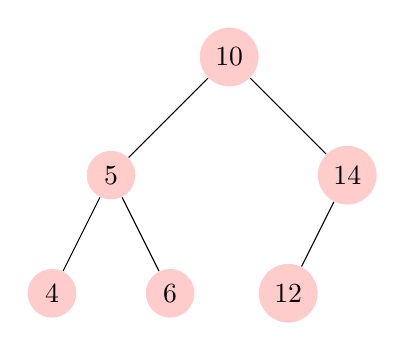
\begin{tikzpicture}[nodes={draw=none,circle,fill=red!20}]
          \node {10}
            child { node {5} 
                child { node {4} }
                child { node {6} }
            }
            child [missing]
            child {node {14} 
                child { node {12} }
                child [missing]
            };
        \end{tikzpicture}
    \end{center}
    \item Selecting $n_{select} = 10$ (root node), Running BFS. \\ Output of BFS $ \leftarrow\{(A, B)\}$ (when ignoring all edge weights less than 10). 
    \item As no path is found between $s = A$ to $t = E$. Selecting $n_{select} = 5$ (left child of node 10). 
    \item Again running BFS, with ignoring all edges with weight less than 5. \\ Output $ \leftarrow\{(A, B), (B, D), (B, C), (D, E)\}$
    \item Path found from A to E. Hence selecting, right child of $n_{select} = 6$.\\ Running BFS again, with ignoring all edges with weight less than 6. \\ Output $ \leftarrow\{(A, B), (B, C), (C, D), (D, E)\}$
    \\ No more child of $n_{select} = 6$. Stopping the loop. 
    \item Final path of minimum edge weight maximized\\
    \textbf{Path} $ \leftarrow\{(A, B), (B, C), (C, D), (D, E)\}$ \\
    \textbf{Minimum Weight (maximized)} $ \leftarrow 6$ 
\end{enumerate}
\end{proof}
\bigskip
\hrule
\bigskip

\end{document}
